% Created by tikzDevice version 0.12
% !TEX encoding = UTF-8 Unicode
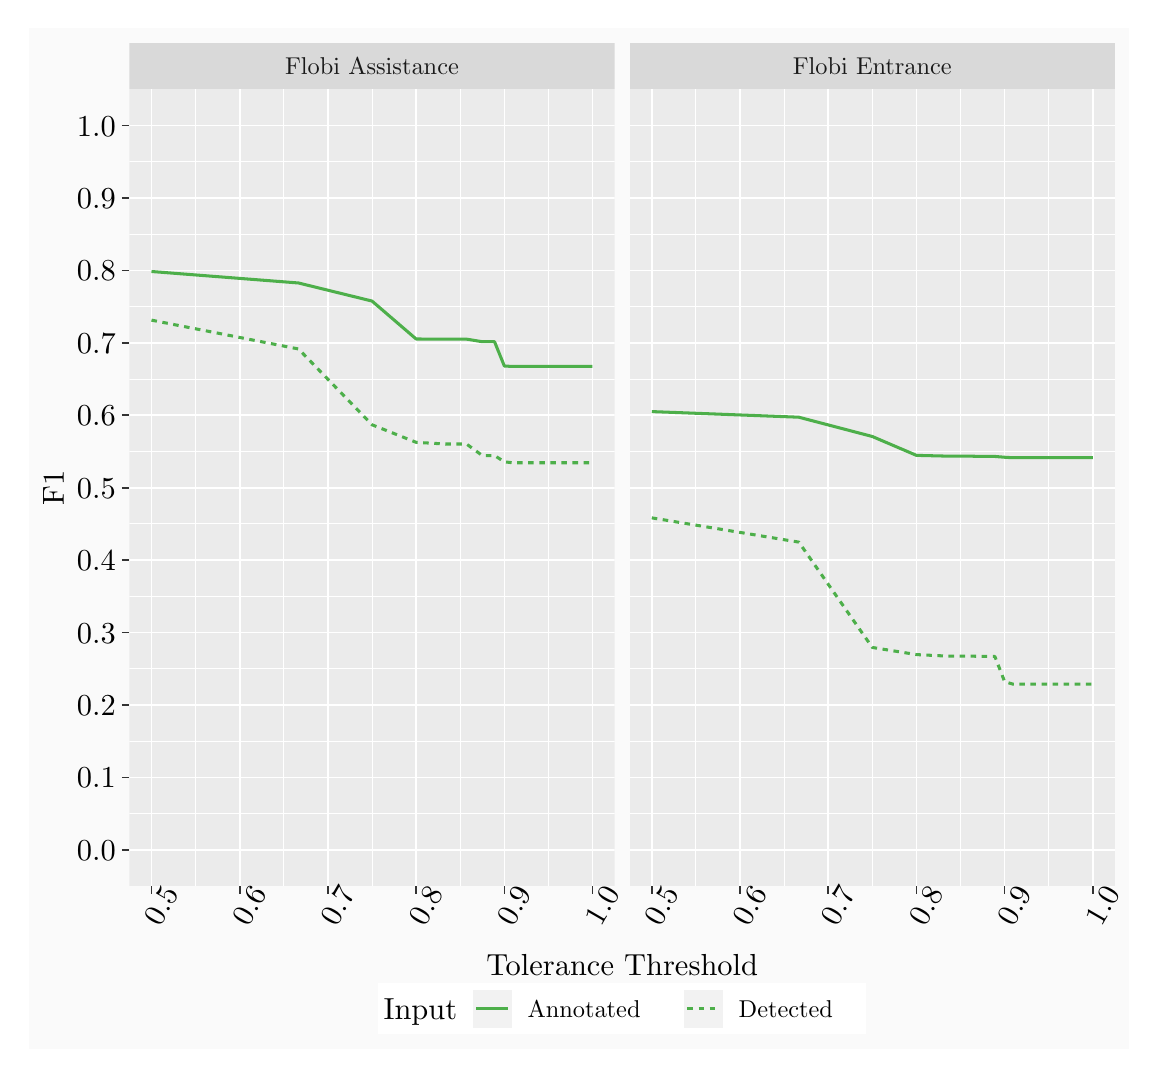
\begin{tikzpicture}[x=1pt,y=1pt]
\definecolor{fillColor}{RGB}{255,255,255}
\path[use as bounding box,fill=fillColor,fill opacity=0.00] (0,0) rectangle (398.34,369.26);
\begin{scope}
\path[clip] (  0.00,  0.00) rectangle (398.34,369.26);
\definecolor{drawColor}{RGB}{255,255,255}
\definecolor{fillColor}{gray}{0.98}

\path[draw=drawColor,line width= 0.6pt,line join=round,line cap=round,fill=fillColor] (  0.00,  0.00) rectangle (398.34,369.26);
\end{scope}
\begin{scope}
\path[clip] ( 36.77, 59.10) rectangle (212.06,346.96);
\definecolor{fillColor}{gray}{0.92}

\path[fill=fillColor] ( 36.77, 59.10) rectangle (212.06,346.96);
\definecolor{drawColor}{RGB}{255,255,255}

\path[draw=drawColor,line width= 0.3pt,line join=round] ( 36.77, 85.27) --
	(212.06, 85.27);

\path[draw=drawColor,line width= 0.3pt,line join=round] ( 36.77,111.44) --
	(212.06,111.44);

\path[draw=drawColor,line width= 0.3pt,line join=round] ( 36.77,137.61) --
	(212.06,137.61);

\path[draw=drawColor,line width= 0.3pt,line join=round] ( 36.77,163.78) --
	(212.06,163.78);

\path[draw=drawColor,line width= 0.3pt,line join=round] ( 36.77,189.95) --
	(212.06,189.95);

\path[draw=drawColor,line width= 0.3pt,line join=round] ( 36.77,216.11) --
	(212.06,216.11);

\path[draw=drawColor,line width= 0.3pt,line join=round] ( 36.77,242.28) --
	(212.06,242.28);

\path[draw=drawColor,line width= 0.3pt,line join=round] ( 36.77,268.45) --
	(212.06,268.45);

\path[draw=drawColor,line width= 0.3pt,line join=round] ( 36.77,294.62) --
	(212.06,294.62);

\path[draw=drawColor,line width= 0.3pt,line join=round] ( 36.77,320.79) --
	(212.06,320.79);

\path[draw=drawColor,line width= 0.3pt,line join=round] ( 60.68, 59.10) --
	( 60.68,346.96);

\path[draw=drawColor,line width= 0.3pt,line join=round] ( 76.62, 59.10) --
	( 76.62,346.96);

\path[draw=drawColor,line width= 0.3pt,line join=round] ( 92.55, 59.10) --
	( 92.55,346.96);

\path[draw=drawColor,line width= 0.3pt,line join=round] (108.49, 59.10) --
	(108.49,346.96);

\path[draw=drawColor,line width= 0.3pt,line join=round] (124.43, 59.10) --
	(124.43,346.96);

\path[draw=drawColor,line width= 0.3pt,line join=round] (156.31, 59.10) --
	(156.31,346.96);

\path[draw=drawColor,line width= 0.3pt,line join=round] (188.18, 59.10) --
	(188.18,346.96);

\path[draw=drawColor,line width= 0.6pt,line join=round] ( 36.77, 72.19) --
	(212.06, 72.19);

\path[draw=drawColor,line width= 0.6pt,line join=round] ( 36.77, 98.36) --
	(212.06, 98.36);

\path[draw=drawColor,line width= 0.6pt,line join=round] ( 36.77,124.52) --
	(212.06,124.52);

\path[draw=drawColor,line width= 0.6pt,line join=round] ( 36.77,150.69) --
	(212.06,150.69);

\path[draw=drawColor,line width= 0.6pt,line join=round] ( 36.77,176.86) --
	(212.06,176.86);

\path[draw=drawColor,line width= 0.6pt,line join=round] ( 36.77,203.03) --
	(212.06,203.03);

\path[draw=drawColor,line width= 0.6pt,line join=round] ( 36.77,229.20) --
	(212.06,229.20);

\path[draw=drawColor,line width= 0.6pt,line join=round] ( 36.77,255.37) --
	(212.06,255.37);

\path[draw=drawColor,line width= 0.6pt,line join=round] ( 36.77,281.53) --
	(212.06,281.53);

\path[draw=drawColor,line width= 0.6pt,line join=round] ( 36.77,307.70) --
	(212.06,307.70);

\path[draw=drawColor,line width= 0.6pt,line join=round] ( 36.77,333.87) --
	(212.06,333.87);

\path[draw=drawColor,line width= 0.6pt,line join=round] ( 44.74, 59.10) --
	( 44.74,346.96);

\path[draw=drawColor,line width= 0.6pt,line join=round] ( 76.62, 59.10) --
	( 76.62,346.96);

\path[draw=drawColor,line width= 0.6pt,line join=round] (108.49, 59.10) --
	(108.49,346.96);

\path[draw=drawColor,line width= 0.6pt,line join=round] (140.37, 59.10) --
	(140.37,346.96);

\path[draw=drawColor,line width= 0.6pt,line join=round] (172.24, 59.10) --
	(172.24,346.96);

\path[draw=drawColor,line width= 0.6pt,line join=round] (204.12, 59.10) --
	(204.12,346.96);
\definecolor{drawColor}{RGB}{77,175,74}

\path[draw=drawColor,line width= 1.1pt,line join=round] ( 44.74,281.15) --
	( 97.87,277.00) --
	(124.43,270.47) --
	(140.37,256.76) --
	(150.99,256.71) --
	(158.58,256.71) --
	(164.27,255.78) --
	(168.70,255.78) --
	(172.24,247.00) --
	(175.14,246.84) --
	(177.56,246.84) --
	(204.09,246.84);

\path[draw=drawColor,line width= 1.1pt,dash pattern=on 2pt off 2pt ,line join=round] ( 44.74,263.57) --
	( 97.87,253.15) --
	(124.43,225.77) --
	(140.37,219.42) --
	(150.99,218.81) --
	(158.58,218.81) --
	(164.27,214.65) --
	(168.70,214.65) --
	(172.24,212.39) --
	(175.14,212.04) --
	(177.56,212.04) --
	(204.09,212.04);
\end{scope}
\begin{scope}
\path[clip] (217.56, 59.10) rectangle (392.84,346.96);
\definecolor{fillColor}{gray}{0.92}

\path[fill=fillColor] (217.56, 59.10) rectangle (392.84,346.96);
\definecolor{drawColor}{RGB}{255,255,255}

\path[draw=drawColor,line width= 0.3pt,line join=round] (217.56, 85.27) --
	(392.84, 85.27);

\path[draw=drawColor,line width= 0.3pt,line join=round] (217.56,111.44) --
	(392.84,111.44);

\path[draw=drawColor,line width= 0.3pt,line join=round] (217.56,137.61) --
	(392.84,137.61);

\path[draw=drawColor,line width= 0.3pt,line join=round] (217.56,163.78) --
	(392.84,163.78);

\path[draw=drawColor,line width= 0.3pt,line join=round] (217.56,189.95) --
	(392.84,189.95);

\path[draw=drawColor,line width= 0.3pt,line join=round] (217.56,216.11) --
	(392.84,216.11);

\path[draw=drawColor,line width= 0.3pt,line join=round] (217.56,242.28) --
	(392.84,242.28);

\path[draw=drawColor,line width= 0.3pt,line join=round] (217.56,268.45) --
	(392.84,268.45);

\path[draw=drawColor,line width= 0.3pt,line join=round] (217.56,294.62) --
	(392.84,294.62);

\path[draw=drawColor,line width= 0.3pt,line join=round] (217.56,320.79) --
	(392.84,320.79);

\path[draw=drawColor,line width= 0.3pt,line join=round] (241.46, 59.10) --
	(241.46,346.96);

\path[draw=drawColor,line width= 0.3pt,line join=round] (257.40, 59.10) --
	(257.40,346.96);

\path[draw=drawColor,line width= 0.3pt,line join=round] (273.34, 59.10) --
	(273.34,346.96);

\path[draw=drawColor,line width= 0.3pt,line join=round] (289.27, 59.10) --
	(289.27,346.96);

\path[draw=drawColor,line width= 0.3pt,line join=round] (305.21, 59.10) --
	(305.21,346.96);

\path[draw=drawColor,line width= 0.3pt,line join=round] (337.09, 59.10) --
	(337.09,346.96);

\path[draw=drawColor,line width= 0.3pt,line join=round] (368.97, 59.10) --
	(368.97,346.96);

\path[draw=drawColor,line width= 0.6pt,line join=round] (217.56, 72.19) --
	(392.84, 72.19);

\path[draw=drawColor,line width= 0.6pt,line join=round] (217.56, 98.36) --
	(392.84, 98.36);

\path[draw=drawColor,line width= 0.6pt,line join=round] (217.56,124.52) --
	(392.84,124.52);

\path[draw=drawColor,line width= 0.6pt,line join=round] (217.56,150.69) --
	(392.84,150.69);

\path[draw=drawColor,line width= 0.6pt,line join=round] (217.56,176.86) --
	(392.84,176.86);

\path[draw=drawColor,line width= 0.6pt,line join=round] (217.56,203.03) --
	(392.84,203.03);

\path[draw=drawColor,line width= 0.6pt,line join=round] (217.56,229.20) --
	(392.84,229.20);

\path[draw=drawColor,line width= 0.6pt,line join=round] (217.56,255.37) --
	(392.84,255.37);

\path[draw=drawColor,line width= 0.6pt,line join=round] (217.56,281.53) --
	(392.84,281.53);

\path[draw=drawColor,line width= 0.6pt,line join=round] (217.56,307.70) --
	(392.84,307.70);

\path[draw=drawColor,line width= 0.6pt,line join=round] (217.56,333.87) --
	(392.84,333.87);

\path[draw=drawColor,line width= 0.6pt,line join=round] (225.52, 59.10) --
	(225.52,346.96);

\path[draw=drawColor,line width= 0.6pt,line join=round] (257.40, 59.10) --
	(257.40,346.96);

\path[draw=drawColor,line width= 0.6pt,line join=round] (289.27, 59.10) --
	(289.27,346.96);

\path[draw=drawColor,line width= 0.6pt,line join=round] (321.15, 59.10) --
	(321.15,346.96);

\path[draw=drawColor,line width= 0.6pt,line join=round] (353.03, 59.10) --
	(353.03,346.96);

\path[draw=drawColor,line width= 0.6pt,line join=round] (384.90, 59.10) --
	(384.90,346.96);
\definecolor{drawColor}{RGB}{77,175,74}

\path[draw=drawColor,line width= 1.1pt,line join=round] (225.52,230.53) --
	(278.65,228.50) --
	(305.21,221.53) --
	(321.15,214.71) --
	(331.78,214.45) --
	(339.37,214.45) --
	(345.06,214.32) --
	(349.49,214.32) --
	(353.03,214.03) --
	(355.92,213.86) --
	(358.34,213.86) --
	(384.87,213.86);

\path[draw=drawColor,line width= 1.1pt,dash pattern=on 2pt off 2pt ,line join=round] (225.52,192.13) --
	(278.65,183.36) --
	(305.21,145.30) --
	(321.15,142.72) --
	(331.78,142.20) --
	(339.37,142.20) --
	(345.06,142.06) --
	(349.49,142.06) --
	(353.03,132.92) --
	(355.92,132.08) --
	(358.34,132.08) --
	(384.87,132.08);
\end{scope}
\begin{scope}
\path[clip] ( 36.77,346.96) rectangle (212.06,363.76);
\definecolor{fillColor}{gray}{0.85}

\path[fill=fillColor] ( 36.77,346.96) rectangle (212.06,363.76);
\definecolor{drawColor}{gray}{0.10}

\node[text=drawColor,anchor=base,inner sep=0pt, outer sep=0pt, scale=  0.88] at (124.41,352.33) {Flobi Assistance};
\end{scope}
\begin{scope}
\path[clip] (217.56,346.96) rectangle (392.84,363.76);
\definecolor{fillColor}{gray}{0.85}

\path[fill=fillColor] (217.56,346.96) rectangle (392.84,363.76);
\definecolor{drawColor}{gray}{0.10}

\node[text=drawColor,anchor=base,inner sep=0pt, outer sep=0pt, scale=  0.88] at (305.20,352.33) {Flobi Entrance};
\end{scope}
\begin{scope}
\path[clip] (  0.00,  0.00) rectangle (398.34,369.26);
\definecolor{drawColor}{gray}{0.20}

\path[draw=drawColor,line width= 0.6pt,line join=round] ( 44.74, 56.35) --
	( 44.74, 59.10);

\path[draw=drawColor,line width= 0.6pt,line join=round] ( 76.62, 56.35) --
	( 76.62, 59.10);

\path[draw=drawColor,line width= 0.6pt,line join=round] (108.49, 56.35) --
	(108.49, 59.10);

\path[draw=drawColor,line width= 0.6pt,line join=round] (140.37, 56.35) --
	(140.37, 59.10);

\path[draw=drawColor,line width= 0.6pt,line join=round] (172.24, 56.35) --
	(172.24, 59.10);

\path[draw=drawColor,line width= 0.6pt,line join=round] (204.12, 56.35) --
	(204.12, 59.10);
\end{scope}
\begin{scope}
\path[clip] (  0.00,  0.00) rectangle (398.34,369.26);
\definecolor{drawColor}{RGB}{0,0,0}

\node[text=drawColor,rotate= 60.00,anchor=base,inner sep=0pt, outer sep=0pt, scale=  1.10] at ( 51.30, 50.37) {0.5};

\node[text=drawColor,rotate= 60.00,anchor=base,inner sep=0pt, outer sep=0pt, scale=  1.10] at ( 83.18, 50.37) {0.6};

\node[text=drawColor,rotate= 60.00,anchor=base,inner sep=0pt, outer sep=0pt, scale=  1.10] at (115.05, 50.37) {0.7};

\node[text=drawColor,rotate= 60.00,anchor=base,inner sep=0pt, outer sep=0pt, scale=  1.10] at (146.93, 50.37) {0.8};

\node[text=drawColor,rotate= 60.00,anchor=base,inner sep=0pt, outer sep=0pt, scale=  1.10] at (178.80, 50.37) {0.9};

\node[text=drawColor,rotate= 60.00,anchor=base,inner sep=0pt, outer sep=0pt, scale=  1.10] at (210.68, 50.37) {1.0};
\end{scope}
\begin{scope}
\path[clip] (  0.00,  0.00) rectangle (398.34,369.26);
\definecolor{drawColor}{gray}{0.20}

\path[draw=drawColor,line width= 0.6pt,line join=round] (225.52, 56.35) --
	(225.52, 59.10);

\path[draw=drawColor,line width= 0.6pt,line join=round] (257.40, 56.35) --
	(257.40, 59.10);

\path[draw=drawColor,line width= 0.6pt,line join=round] (289.27, 56.35) --
	(289.27, 59.10);

\path[draw=drawColor,line width= 0.6pt,line join=round] (321.15, 56.35) --
	(321.15, 59.10);

\path[draw=drawColor,line width= 0.6pt,line join=round] (353.03, 56.35) --
	(353.03, 59.10);

\path[draw=drawColor,line width= 0.6pt,line join=round] (384.90, 56.35) --
	(384.90, 59.10);
\end{scope}
\begin{scope}
\path[clip] (  0.00,  0.00) rectangle (398.34,369.26);
\definecolor{drawColor}{RGB}{0,0,0}

\node[text=drawColor,rotate= 60.00,anchor=base,inner sep=0pt, outer sep=0pt, scale=  1.10] at (232.08, 50.37) {0.5};

\node[text=drawColor,rotate= 60.00,anchor=base,inner sep=0pt, outer sep=0pt, scale=  1.10] at (263.96, 50.37) {0.6};

\node[text=drawColor,rotate= 60.00,anchor=base,inner sep=0pt, outer sep=0pt, scale=  1.10] at (295.84, 50.37) {0.7};

\node[text=drawColor,rotate= 60.00,anchor=base,inner sep=0pt, outer sep=0pt, scale=  1.10] at (327.71, 50.37) {0.8};

\node[text=drawColor,rotate= 60.00,anchor=base,inner sep=0pt, outer sep=0pt, scale=  1.10] at (359.59, 50.37) {0.9};

\node[text=drawColor,rotate= 60.00,anchor=base,inner sep=0pt, outer sep=0pt, scale=  1.10] at (391.46, 50.37) {1.0};
\end{scope}
\begin{scope}
\path[clip] (  0.00,  0.00) rectangle (398.34,369.26);
\definecolor{drawColor}{RGB}{0,0,0}

\node[text=drawColor,anchor=base east,inner sep=0pt, outer sep=0pt, scale=  1.10] at ( 31.82, 68.40) {0.0};

\node[text=drawColor,anchor=base east,inner sep=0pt, outer sep=0pt, scale=  1.10] at ( 31.82, 94.57) {0.1};

\node[text=drawColor,anchor=base east,inner sep=0pt, outer sep=0pt, scale=  1.10] at ( 31.82,120.74) {0.2};

\node[text=drawColor,anchor=base east,inner sep=0pt, outer sep=0pt, scale=  1.10] at ( 31.82,146.90) {0.3};

\node[text=drawColor,anchor=base east,inner sep=0pt, outer sep=0pt, scale=  1.10] at ( 31.82,173.07) {0.4};

\node[text=drawColor,anchor=base east,inner sep=0pt, outer sep=0pt, scale=  1.10] at ( 31.82,199.24) {0.5};

\node[text=drawColor,anchor=base east,inner sep=0pt, outer sep=0pt, scale=  1.10] at ( 31.82,225.41) {0.6};

\node[text=drawColor,anchor=base east,inner sep=0pt, outer sep=0pt, scale=  1.10] at ( 31.82,251.58) {0.7};

\node[text=drawColor,anchor=base east,inner sep=0pt, outer sep=0pt, scale=  1.10] at ( 31.82,277.75) {0.8};

\node[text=drawColor,anchor=base east,inner sep=0pt, outer sep=0pt, scale=  1.10] at ( 31.82,303.91) {0.9};

\node[text=drawColor,anchor=base east,inner sep=0pt, outer sep=0pt, scale=  1.10] at ( 31.82,330.08) {1.0};
\end{scope}
\begin{scope}
\path[clip] (  0.00,  0.00) rectangle (398.34,369.26);
\definecolor{drawColor}{gray}{0.20}

\path[draw=drawColor,line width= 0.6pt,line join=round] ( 34.02, 72.19) --
	( 36.77, 72.19);

\path[draw=drawColor,line width= 0.6pt,line join=round] ( 34.02, 98.36) --
	( 36.77, 98.36);

\path[draw=drawColor,line width= 0.6pt,line join=round] ( 34.02,124.52) --
	( 36.77,124.52);

\path[draw=drawColor,line width= 0.6pt,line join=round] ( 34.02,150.69) --
	( 36.77,150.69);

\path[draw=drawColor,line width= 0.6pt,line join=round] ( 34.02,176.86) --
	( 36.77,176.86);

\path[draw=drawColor,line width= 0.6pt,line join=round] ( 34.02,203.03) --
	( 36.77,203.03);

\path[draw=drawColor,line width= 0.6pt,line join=round] ( 34.02,229.20) --
	( 36.77,229.20);

\path[draw=drawColor,line width= 0.6pt,line join=round] ( 34.02,255.37) --
	( 36.77,255.37);

\path[draw=drawColor,line width= 0.6pt,line join=round] ( 34.02,281.53) --
	( 36.77,281.53);

\path[draw=drawColor,line width= 0.6pt,line join=round] ( 34.02,307.70) --
	( 36.77,307.70);

\path[draw=drawColor,line width= 0.6pt,line join=round] ( 34.02,333.87) --
	( 36.77,333.87);
\end{scope}
\begin{scope}
\path[clip] (  0.00,  0.00) rectangle (398.34,369.26);
\definecolor{drawColor}{RGB}{0,0,0}

\node[text=drawColor,anchor=base,inner sep=0pt, outer sep=0pt, scale=  1.10] at (214.81, 26.90) {Tolerance Threshold};
\end{scope}
\begin{scope}
\path[clip] (  0.00,  0.00) rectangle (398.34,369.26);
\definecolor{drawColor}{RGB}{0,0,0}

\node[text=drawColor,rotate= 90.00,anchor=base,inner sep=0pt, outer sep=0pt, scale=  1.10] at ( 13.08,203.03) {F1};
\end{scope}
\begin{scope}
\path[clip] (  0.00,  0.00) rectangle (398.34,369.26);
\definecolor{fillColor}{RGB}{255,255,255}

\path[fill=fillColor] (126.61,  5.50) rectangle (303.00, 23.95);
\end{scope}
\begin{scope}
\path[clip] (  0.00,  0.00) rectangle (398.34,369.26);
\definecolor{drawColor}{RGB}{0,0,0}

\node[text=drawColor,anchor=base west,inner sep=0pt, outer sep=0pt, scale=  1.10] at (128.61, 10.94) {Input};
\end{scope}
\begin{scope}
\path[clip] (  0.00,  0.00) rectangle (398.34,369.26);
\definecolor{drawColor}{RGB}{255,255,255}
\definecolor{fillColor}{gray}{0.95}

\path[draw=drawColor,line width= 0.6pt,line join=round,line cap=round,fill=fillColor] (160.69,  7.50) rectangle (175.14, 21.95);
\end{scope}
\begin{scope}
\path[clip] (  0.00,  0.00) rectangle (398.34,369.26);
\definecolor{drawColor}{RGB}{77,175,74}

\path[draw=drawColor,line width= 1.1pt,line join=round] (162.13, 14.73) -- (173.70, 14.73);
\end{scope}
\begin{scope}
\path[clip] (  0.00,  0.00) rectangle (398.34,369.26);
\definecolor{drawColor}{RGB}{255,255,255}
\definecolor{fillColor}{gray}{0.95}

\path[draw=drawColor,line width= 0.6pt,line join=round,line cap=round,fill=fillColor] (236.95,  7.50) rectangle (251.41, 21.95);
\end{scope}
\begin{scope}
\path[clip] (  0.00,  0.00) rectangle (398.34,369.26);
\definecolor{drawColor}{RGB}{77,175,74}

\path[draw=drawColor,line width= 1.1pt,dash pattern=on 2pt off 2pt ,line join=round] (238.40, 14.73) -- (249.96, 14.73);
\end{scope}
\begin{scope}
\path[clip] (  0.00,  0.00) rectangle (398.34,369.26);
\definecolor{drawColor}{RGB}{0,0,0}

\node[text=drawColor,anchor=base west,inner sep=0pt, outer sep=0pt, scale=  0.88] at (180.64, 11.70) {Annotated};
\end{scope}
\begin{scope}
\path[clip] (  0.00,  0.00) rectangle (398.34,369.26);
\definecolor{drawColor}{RGB}{0,0,0}

\node[text=drawColor,anchor=base west,inner sep=0pt, outer sep=0pt, scale=  0.88] at (256.91, 11.70) {Detected};
\end{scope}
\end{tikzpicture}
